\documentclass[crop,tikz]{standalone}
\usetikzlibrary{backgrounds}
\colorlet{blue}{cyan}
\tikzset{ inverted/.style={every path/.style={draw=white,text=white}, background rectangle/.style={fill}, show background rectangle }}

\tikzset{>=latex}
\usetikzlibrary{calc}
\colorlet{green}{green}
\newcommand{\place}{\vec{r}}

\begin{document}
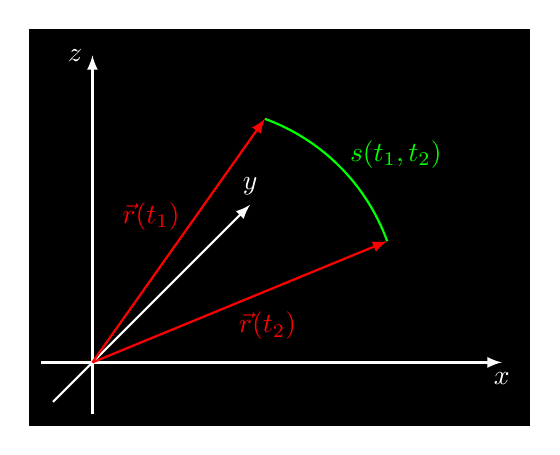
\begin{tikzpicture}[inverted,scale=1.3]
  % axes
  \draw[->,thick] (xyz cs:x=-0.5) -- (xyz cs:x=4)  node[below] {$x$};
  \draw[->,thick] (xyz cs:y=-0.5) -- (xyz cs:y=3)  node[left] {$z$};
  \draw[->,thick] (xyz cs:z=1)    -- (xyz cs:z=-4) node[above] {$y$};
  % space point
  \coordinate (r1) at ($(1,0.5)+(70:2)$);
  \coordinate (r2) at ($(1,0.5)+(20:2)$);
  % path
  \draw[thick,green] (r1) arc (70:20:2);
  \node[right,xshift=0.5em,green] at ($(1,0.5)+(50:2)$) {$s(t_1,t_2)$};
  % space-point vectors
  \draw[->,thick,red] (xyz cs:x=0) -- node[above,xshift=-1em]{$\place(t_1)$} (r1);
  \draw[->,thick,red] (xyz cs:x=0) -- node[below,xshift=+1em]{$\place(t_2)$} (r2);
\end{tikzpicture}
\end{document}
